\begin{figure}
    \begin{center}
        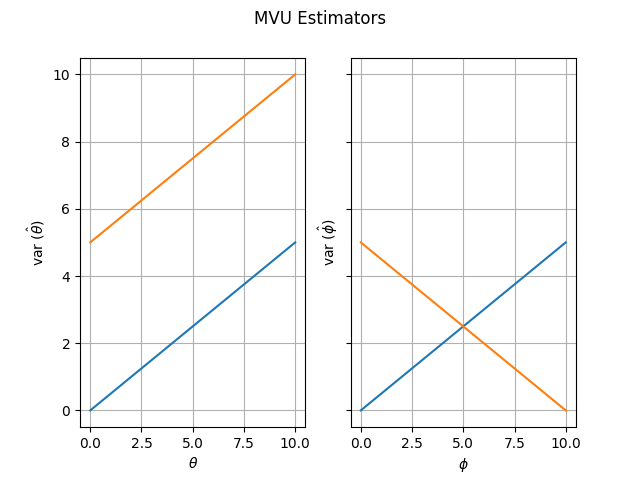
\includegraphics[width=0.6\textwidth]{assets/mvu.png}
    \end{center}
    \label{fig:mvu}
\end{figure}

An estimator is said to be unbiased when on average the estimator yields the true value for any range of values that the estimated parameter can take. Mathematically, this can be written as shown in equation \ref{eq:unbiased_single} where $g(\mathbf{x})$ is the estimator.

\begin{equation}
    \mathcal{E}(\hat{\theta}) = \int g(\mathbf{x}) p(\mathbf{x}; \theta) d\mathbf{x} = \theta \qquad \forall \qquad \theta \in \left(a, b\right)
    \label{eq:unbiased_single}
\end{equation}

The same in vector form can be defined as shown in equation \ref{eq:unbiased_vector} if the parameter $\mathbf{\theta} = \left[\theta_1 \theta_2 \hdots \theta_N\right]^T$ is estimated using an estimator defined as $\mathbf{\hat{\theta}} = \left[\hat{\theta}_1 \hat{\theta}_2 \hdots \hat{\theta}_N\right]^T$. If we define the expected value of a vector to be the expected value of its components then it can also be written in vector form.

\begin{equation}
    \begin{split}
        \mathcal{E}(\hat{\theta_i}) &= \theta_i \qquad \forall \qquad \theta_i \in \left(a_i, b_i\right) \\
        \mathcal{E}(\hat{\mathbf{\theta}}) &= \mathbf{\theta}
    \end{split}
    \label{eq:unbiased_vector}
\end{equation}

An unbiased estimator does not imply a good estimator but only that it converges on average to the true value. However, an biased estimator always leads to poor results. Therefore, to judge the quality of an estimator, we would need to define some optimality criterion.

\subsection{Minimize the Mean Square Error?}

A natural choice for the optimality is the estimtaor that minimizes the \textbf{mean square error}. However, these estimators are generally difficult to find. Consider the mean square error are shown in equation \ref{eq:mvu_case}. One way of finding the estimator could be to assign the first derivative of this equation to $0$ which might yield the optimal estimator. However, this result would depend on the parameter $\theta$ to be estimated which makes it a chicken or egg problem. Therefore a minimum MSE estimator in most cases is unrealizable.

\begin{equation}
    \begin{split}
        \text{mse}(\hat{\mathbf{\theta}}) &= \mathcal{E}\left\{(\hat{\theta} - \theta)^2\right\} \\
        &= \mathcal{E} \left\{\hat{\theta}^2 + \theta^2 + 2\hat{\theta}\theta\right\} \\
        &= \mathcal{E}(\hat{\theta}^2) + \theta^2 + 2\mathcal{E}(\hat{\theta})\theta
    \end{split}
    \label{eq:mvu_case}
\end{equation}

\subsection{Alternative: Minimum Variance Unbiased Estimator}

Another approach is to make sure that the estimator is unbiased and them minimizing its variance. The question now is whether such an estimator exists. In general, the MVU does not always exist as the best MVU \textbf{could} depend no the value of the parameter that is to be estimated. This is seen in figure \ref{fig:mvu} where $\theta$ has a realizable MVU estimator and $\phi$ doesn't. Even if it does exist, sometimes the best estimator cannot be found. Therefore, three possible approaches can be taken:

\begin{itemize}
    \item Determine Cramer-Rao Lower Bound (CRLB) $\longrightarrow$ Find Estimator that satisfies it
    \item Apply the Rao-Blackwell-Lehmann-Scheffe (RBLS) Theorem
    \item Restrict the Estimator to be \textbf{Linear} as well as Unbiased. This helps reduce the search space to find an Estimator
\end{itemize}